% ==============================================================================
% PROFESSIONAL ERD: Dual Indexing Schema (Neo4j + Milvus)
% Requires: \usepackage{tikz}
%           \usetikzlibrary{positioning, arrows.meta, fit, backgrounds, calc}
% ==============================================================================

\documentclass[tikz,border=15pt]{standalone}
\usepackage[T1]{fontenc}
\usepackage{lmodern}
\usetikzlibrary{positioning, arrows.meta, fit, backgrounds, calc}

\begin{document}

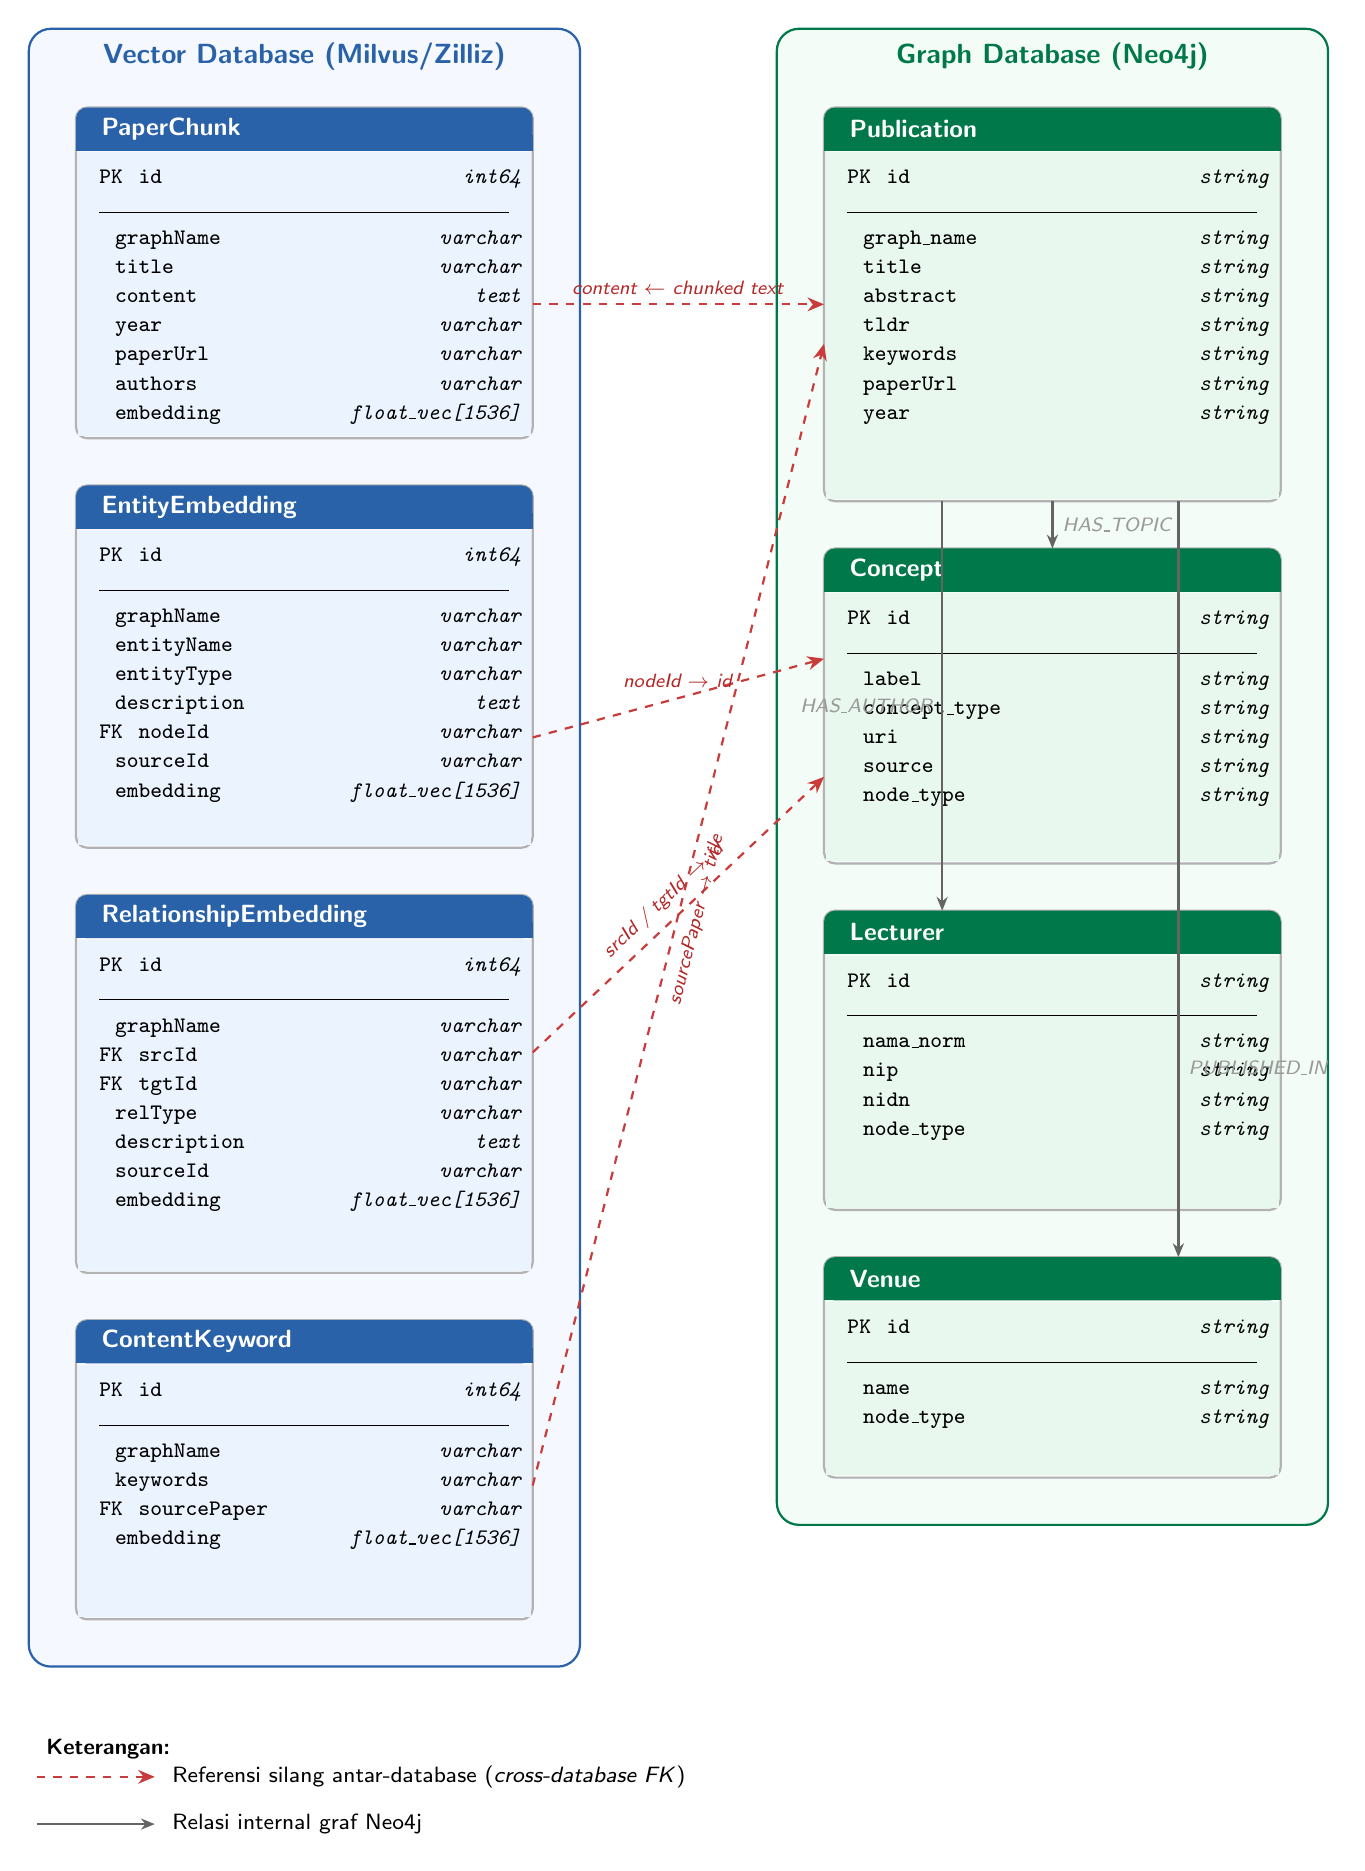
\begin{tikzpicture}[
    % === COLOR DEFINITIONS ===
    milvus header/.style={fill={rgb,255:red,41;green,98;blue,168}},      % Deep blue
    neo4j header/.style={fill={rgb,255:red,0;green,120;blue,74}},        % Neo4j green
    milvus body/.style={fill={rgb,255:red,235;green,243;blue,255}},      % Light blue
    neo4j body/.style={fill={rgb,255:red,232;green,248;blue,239}},       % Light green
    milvus group bg/.style={fill={rgb,255:red,245;green,249;blue,255}},  % Very light blue
    neo4j group bg/.style={fill={rgb,255:red,243;green,252;blue,246}},   % Very light green
    % === ARROW STYLES ===
    fk arrow/.style={
        draw={rgb,255:red,200;green,60;blue,60},
        thick,
        dashed,
        -{Stealth[length=6pt, width=5pt]},
    },
    graph rel/.style={
        draw={rgb,255:red,100;green,100;blue,100},
        thick,
        -{Stealth[length=5pt, width=4pt]},
    },
]

% ================================================================
% HELPER: Entity table macro
% Args: #1=name, #2=header style, #3=body style, #4=fields
% ================================================================
% We'll draw entities manually for full control

% ================================================================
% MILVUS ENTITIES (Left Side)
% ================================================================

% --- PaperChunk ---
\node[anchor=north west] (pc_title) at (0, 0) {};
\draw[rounded corners=4pt, thick, draw=gray!60]
    (0, 0) rectangle (5.8, -4.2);
\fill[milvus header, rounded corners=4pt]
    (0, 0) rectangle (5.8, -0.55);
\fill[milvus header]
    (0, -0.35) rectangle (5.8, -0.55);
\node[font=\small\bfseries\sffamily, text=white, anchor=west] at (0.2, -0.275) {PaperChunk};
\fill[milvus body]
    (0.02, -0.57) rectangle (5.78, -4.17);
\node[font=\footnotesize\ttfamily, anchor=north west, text width=5.4cm, inner sep=4pt] at (0.15, -0.65) {
    \textbf{PK}~~id \hfill \textit{int64}\\[1pt]
    \rule{5.2cm}{0.3pt}\\[2pt]
    ~~graphName \hfill \textit{varchar}\\[1pt]
    ~~title \hfill \textit{varchar}\\[1pt]
    ~~content \hfill \textit{text}\\[1pt]
    ~~year \hfill \textit{varchar}\\[1pt]
    ~~paperUrl \hfill \textit{varchar}\\[1pt]
    ~~authors \hfill \textit{varchar}\\[1pt]
    ~~embedding \hfill \textit{float\_vec[1536]}
};

% --- EntityEmbedding ---
\draw[rounded corners=4pt, thick, draw=gray!60]
    (0, -4.8) rectangle (5.8, -9.4);
\fill[milvus header, rounded corners=4pt]
    (0, -4.8) rectangle (5.8, -5.35);
\fill[milvus header]
    (0, -5.15) rectangle (5.8, -5.35);
\node[font=\small\bfseries\sffamily, text=white, anchor=west] at (0.2, -5.075) {EntityEmbedding};
\fill[milvus body]
    (0.02, -5.37) rectangle (5.78, -9.37);
\node[font=\footnotesize\ttfamily, anchor=north west, text width=5.4cm, inner sep=4pt] at (0.15, -5.45) {
    \textbf{PK}~~id \hfill \textit{int64}\\[1pt]
    \rule{5.2cm}{0.3pt}\\[2pt]
    ~~graphName \hfill \textit{varchar}\\[1pt]
    ~~entityName \hfill \textit{varchar}\\[1pt]
    ~~entityType \hfill \textit{varchar}\\[1pt]
    ~~description \hfill \textit{text}\\[1pt]
    \textbf{FK}~~nodeId \hfill \textit{varchar}\\[1pt]
    ~~sourceId \hfill \textit{varchar}\\[1pt]
    ~~embedding \hfill \textit{float\_vec[1536]}
};

% --- RelationshipEmbedding ---
\draw[rounded corners=4pt, thick, draw=gray!60]
    (0, -10.0) rectangle (5.8, -14.8);
\fill[milvus header, rounded corners=4pt]
    (0, -10.0) rectangle (5.8, -10.55);
\fill[milvus header]
    (0, -10.35) rectangle (5.8, -10.55);
\node[font=\small\bfseries\sffamily, text=white, anchor=west] at (0.2, -10.275) {RelationshipEmbedding};
\fill[milvus body]
    (0.02, -10.57) rectangle (5.78, -14.77);
\node[font=\footnotesize\ttfamily, anchor=north west, text width=5.4cm, inner sep=4pt] at (0.15, -10.65) {
    \textbf{PK}~~id \hfill \textit{int64}\\[1pt]
    \rule{5.2cm}{0.3pt}\\[2pt]
    ~~graphName \hfill \textit{varchar}\\[1pt]
    \textbf{FK}~~srcId \hfill \textit{varchar}\\[1pt]
    \textbf{FK}~~tgtId \hfill \textit{varchar}\\[1pt]
    ~~relType \hfill \textit{varchar}\\[1pt]
    ~~description \hfill \textit{text}\\[1pt]
    ~~sourceId \hfill \textit{varchar}\\[1pt]
    ~~embedding \hfill \textit{float\_vec[1536]}
};

% --- ContentKeyword ---
\draw[rounded corners=4pt, thick, draw=gray!60]
    (0, -15.4) rectangle (5.8, -19.2);
\fill[milvus header, rounded corners=4pt]
    (0, -15.4) rectangle (5.8, -15.95);
\fill[milvus header]
    (0, -15.75) rectangle (5.8, -15.95);
\node[font=\small\bfseries\sffamily, text=white, anchor=west] at (0.2, -15.675) {ContentKeyword};
\fill[milvus body]
    (0.02, -15.97) rectangle (5.78, -19.17);
\node[font=\footnotesize\ttfamily, anchor=north west, text width=5.4cm, inner sep=4pt] at (0.15, -16.05) {
    \textbf{PK}~~id \hfill \textit{int64}\\[1pt]
    \rule{5.2cm}{0.3pt}\\[2pt]
    ~~graphName \hfill \textit{varchar}\\[1pt]
    ~~keywords \hfill \textit{varchar}\\[1pt]
    \textbf{FK}~~sourcePaper \hfill \textit{varchar}\\[1pt]
    ~~embedding \hfill \textit{float\_vec[1536]}
};

% ================================================================
% NEO4J ENTITIES (Right Side)
% ================================================================

% --- Publication ---
\draw[rounded corners=4pt, thick, draw=gray!60]
    (9.5, 0) rectangle (15.3, -5.0);
\fill[neo4j header, rounded corners=4pt]
    (9.5, 0) rectangle (15.3, -0.55);
\fill[neo4j header]
    (9.5, -0.35) rectangle (15.3, -0.55);
\node[font=\small\bfseries\sffamily, text=white, anchor=west] at (9.7, -0.275) {Publication};
\fill[neo4j body]
    (9.52, -0.57) rectangle (15.28, -4.97);
\node[font=\footnotesize\ttfamily, anchor=north west, text width=5.4cm, inner sep=4pt] at (9.65, -0.65) {
    \textbf{PK}~~id \hfill \textit{string}\\[1pt]
    \rule{5.2cm}{0.3pt}\\[2pt]
    ~~graph\_name \hfill \textit{string}\\[1pt]
    ~~title \hfill \textit{string}\\[1pt]
    ~~abstract \hfill \textit{string}\\[1pt]
    ~~tldr \hfill \textit{string}\\[1pt]
    ~~keywords \hfill \textit{string}\\[1pt]
    ~~paperUrl \hfill \textit{string}\\[1pt]
    ~~year \hfill \textit{string}
};

% --- Concept ---
\draw[rounded corners=4pt, thick, draw=gray!60]
    (9.5, -5.6) rectangle (15.3, -9.6);
\fill[neo4j header, rounded corners=4pt]
    (9.5, -5.6) rectangle (15.3, -6.15);
\fill[neo4j header]
    (9.5, -5.95) rectangle (15.3, -6.15);
\node[font=\small\bfseries\sffamily, text=white, anchor=west] at (9.7, -5.875) {Concept};
\fill[neo4j body]
    (9.52, -6.17) rectangle (15.28, -9.57);
\node[font=\footnotesize\ttfamily, anchor=north west, text width=5.4cm, inner sep=4pt] at (9.65, -6.25) {
    \textbf{PK}~~id \hfill \textit{string}\\[1pt]
    \rule{5.2cm}{0.3pt}\\[2pt]
    ~~label \hfill \textit{string}\\[1pt]
    ~~concept\_type \hfill \textit{string}\\[1pt]
    ~~uri \hfill \textit{string}\\[1pt]
    ~~source \hfill \textit{string}\\[1pt]
    ~~node\_type \hfill \textit{string}
};

% --- Lecturer ---
\draw[rounded corners=4pt, thick, draw=gray!60]
    (9.5, -10.2) rectangle (15.3, -14.0);
\fill[neo4j header, rounded corners=4pt]
    (9.5, -10.2) rectangle (15.3, -10.75);
\fill[neo4j header]
    (9.5, -10.55) rectangle (15.3, -10.75);
\node[font=\small\bfseries\sffamily, text=white, anchor=west] at (9.7, -10.475) {Lecturer};
\fill[neo4j body]
    (9.52, -10.77) rectangle (15.28, -13.97);
\node[font=\footnotesize\ttfamily, anchor=north west, text width=5.4cm, inner sep=4pt] at (9.65, -10.85) {
    \textbf{PK}~~id \hfill \textit{string}\\[1pt]
    \rule{5.2cm}{0.3pt}\\[2pt]
    ~~nama\_norm \hfill \textit{string}\\[1pt]
    ~~nip \hfill \textit{string}\\[1pt]
    ~~nidn \hfill \textit{string}\\[1pt]
    ~~node\_type \hfill \textit{string}
};

% --- Venue ---
\draw[rounded corners=4pt, thick, draw=gray!60]
    (9.5, -14.6) rectangle (15.3, -17.4);
\fill[neo4j header, rounded corners=4pt]
    (9.5, -14.6) rectangle (15.3, -15.15);
\fill[neo4j header]
    (9.5, -14.95) rectangle (15.3, -15.15);
\node[font=\small\bfseries\sffamily, text=white, anchor=west] at (9.7, -14.875) {Venue};
\fill[neo4j body]
    (9.52, -15.17) rectangle (15.28, -17.37);
\node[font=\footnotesize\ttfamily, anchor=north west, text width=5.4cm, inner sep=4pt] at (9.65, -15.25) {
    \textbf{PK}~~id \hfill \textit{string}\\[1pt]
    \rule{5.2cm}{0.3pt}\\[2pt]
    ~~name \hfill \textit{string}\\[1pt]
    ~~node\_type \hfill \textit{string}
};

% ================================================================
% GROUP BACKGROUNDS
% ================================================================
\begin{scope}[on background layer]
    % Milvus group
    \fill[milvus group bg, rounded corners=8pt]
        (-0.6, 1.0) rectangle (6.4, -19.8);
    \draw[draw={rgb,255:red,41;green,98;blue,168}, thick, rounded corners=8pt]
        (-0.6, 1.0) rectangle (6.4, -19.8);
    % Neo4j group
    \fill[neo4j group bg, rounded corners=8pt]
        (8.9, 1.0) rectangle (15.9, -18.0);
    \draw[draw={rgb,255:red,0;green,120;blue,74}, thick, rounded corners=8pt]
        (8.9, 1.0) rectangle (15.9, -18.0);
\end{scope}

% ================================================================
% GROUP LABELS
% ================================================================
\node[font=\normalsize\bfseries\sffamily, text={rgb,255:red,41;green,98;blue,168}]
    at (2.9, 0.65) {Vector Database (Milvus/Zilliz)};
\node[font=\normalsize\bfseries\sffamily, text={rgb,255:red,0;green,120;blue,74}]
    at (12.4, 0.65) {Graph Database (Neo4j)};

% ================================================================
% CROSS-DATABASE RELATIONSHIPS (FK Arrows)
% ================================================================

% EntityEmbedding.nodeId --> Concept.id
\draw[fk arrow]
    (5.8, -8.0) -- node[above, font=\scriptsize\sffamily, text={rgb,255:red,180;green,40;blue,40}]
    {\textit{nodeId $\rightarrow$ id}} (9.5, -7.0);

% RelationshipEmbedding.srcId --> Concept.id
\draw[fk arrow]
    (5.8, -12.0) -- node[above, sloped, font=\scriptsize\sffamily, text={rgb,255:red,180;green,40;blue,40}]
    {\textit{srcId / tgtId $\rightarrow$ id}} (9.5, -8.5);

% ContentKeyword.sourcePaper --> Publication.title
\draw[fk arrow]
    (5.8, -17.5) -- node[below, sloped, font=\scriptsize\sffamily, text={rgb,255:red,180;green,40;blue,40}]
    {\textit{sourcePaper $\rightarrow$ title}} (9.5, -3.0);

% PaperChunk.content --> Publication (content mapping)
\draw[fk arrow]
    (5.8, -2.5) -- node[above, font=\scriptsize\sffamily, text={rgb,255:red,180;green,40;blue,40}]
    {\textit{content $\leftarrow$ chunked text}} (9.5, -2.5);

% ================================================================
% NEO4J INTERNAL RELATIONSHIPS
% ================================================================

% Publication -> Concept (HAS_TOPIC)
\draw[graph rel]
    (12.4, -5.0) -- node[right, font=\scriptsize\sffamily\itshape, text=gray!80]
    {HAS\_TOPIC} (12.4, -5.6);

% Publication -> Lecturer (HAS_AUTHOR)
\draw[graph rel]
    (11.0, -5.0) -- node[left, font=\scriptsize\sffamily\itshape, text=gray!80]
    {HAS\_AUTHOR} (11.0, -10.2);

% Publication -> Venue (PUBLISHED_IN)
\draw[graph rel]
    (14.0, -5.0) -- node[right, font=\scriptsize\sffamily\itshape, text=gray!80, near end]
    {PUBLISHED\_IN} (14.0, -14.6);

% ================================================================
% LEGEND
% ================================================================
\node[anchor=north west, font=\footnotesize\sffamily] at (-0.5, -20.6) {
    \textbf{Keterangan:}
};
\draw[fk arrow] (-0.5, -21.2) -- (1.0, -21.2);
\node[anchor=west, font=\footnotesize\sffamily] at (1.1, -21.2)
    {Referensi silang antar-database (\textit{cross-database FK})};
\draw[graph rel] (-0.5, -21.8) -- (1.0, -21.8);
\node[anchor=west, font=\footnotesize\sffamily] at (1.1, -21.8)
    {Relasi internal graf Neo4j};

\end{tikzpicture}

\end{document}
